%%%
%
% $Autor: Müller, Hinrichs $
% $Datum: 2026-06-09 14:18:35Z $
% $Pfad: UltraschallradarAutomatisierungstechnik/report/Contents/General/Systementwicklung.tex $
% $Version: 1 $
%
% Project: 
%
%%%


\chapter{Mechatronische Systementwicklung und Implementierung}
\label{chap:Development_Umsetzung}

Dieses Kapitel dokumentiert die praktische Umsetzung des Ultraschallradarsystems. Es beschreibt den Entwicklungsprozess von der Definition der Systemarchitektur über die Konstruktion des Gehäuses in CAD bis hin zur  Fertigung des Systems.

\section{Systemarchitektur}
\label{sec:Systemarchitektur_Workflow}

Zu Beginn des Projekts wurde eine  Anforderungsliste definiert, wie das Ultraschallradarsystem umzusetzen ist. Das System muss kompakt, transportabel, plattformunabhängig einsetzbar sowie unempfindlich gegenüber Dauerbetrieb sein. Zusätzlich muss der Benutzer den Zustand des Systems immer erkennen können.

Die funktionale Aufteilung der Komponenten gliedert sich wie folgt:
\begin{itemize}
	\item \textbf{Aktorik (Mechanische Ebene):} Ein Servomotor des Typs TowerPro SG90 übernimmt die winkelgesteuerte Positionierung der Sensorplattform in einem Bereich von 120$^\circ$ (30$^\circ$ bis 150$^\circ$).
	\item \textbf{Sensorik (Elektronische Ebene):} Der Ultraschallsensor HC-SR04 erfasst die Echolaufzeit von Objekten im Nahbereich.
	\item \textbf{Visualisierung (Status-LED's):} Zwei im Gehäuse integrierte Status-LED's (rot und grün) geben kontinuierlich den Zustand des Systems wieder.
	\item \textbf{Steuerung (Embedded Software):} Ein Arduino-Mikrocontroller verarbeitet die Hardware-Schnittstellen, steuert den Servomotor per Pulsweitenmodulation (PWM) an und überträgt die Daten über die serielle USB-Schnittstelle.
	\item \textbf{Visualisierung (Applikation):} Eine in Processing 4.3 entwickelte Desktop-Anwendung übernimmt die Darstellung und Filterung der Messergebnisse.
\end{itemize}

\section{Konstruktive Auslegung und CAD-Entwicklung (SolidWorks)}
\label{sec:CAD_Entwicklung_Detailliert}

Die Konstruktion des Radarsystems wurde modular in einer CAD-Umgebung umgesetzt, um eine exakte Passgenauigkeit vor der additiven Fertigung zu garantieren. Das Gesamtsystem ist für maximale Portabilität auf kompakte Au\ss enabmessungen von $80 \times 80 \times 100\text{ mm}$ (Breite $\times$ Tiefe $\times$ Höhe) dimensioniert. Um eine hohe mechanische Steifigkeit gegenüber Verwindungen zu garantieren und gleichzeitig das Innenvolumen zu maximieren, wurde für sämtliche Gehäusekomponenten eine homogene Wandstärke von $2{,}5\text{ mm}$ definiert.

\begin{figure}[htbp]
	\centering
	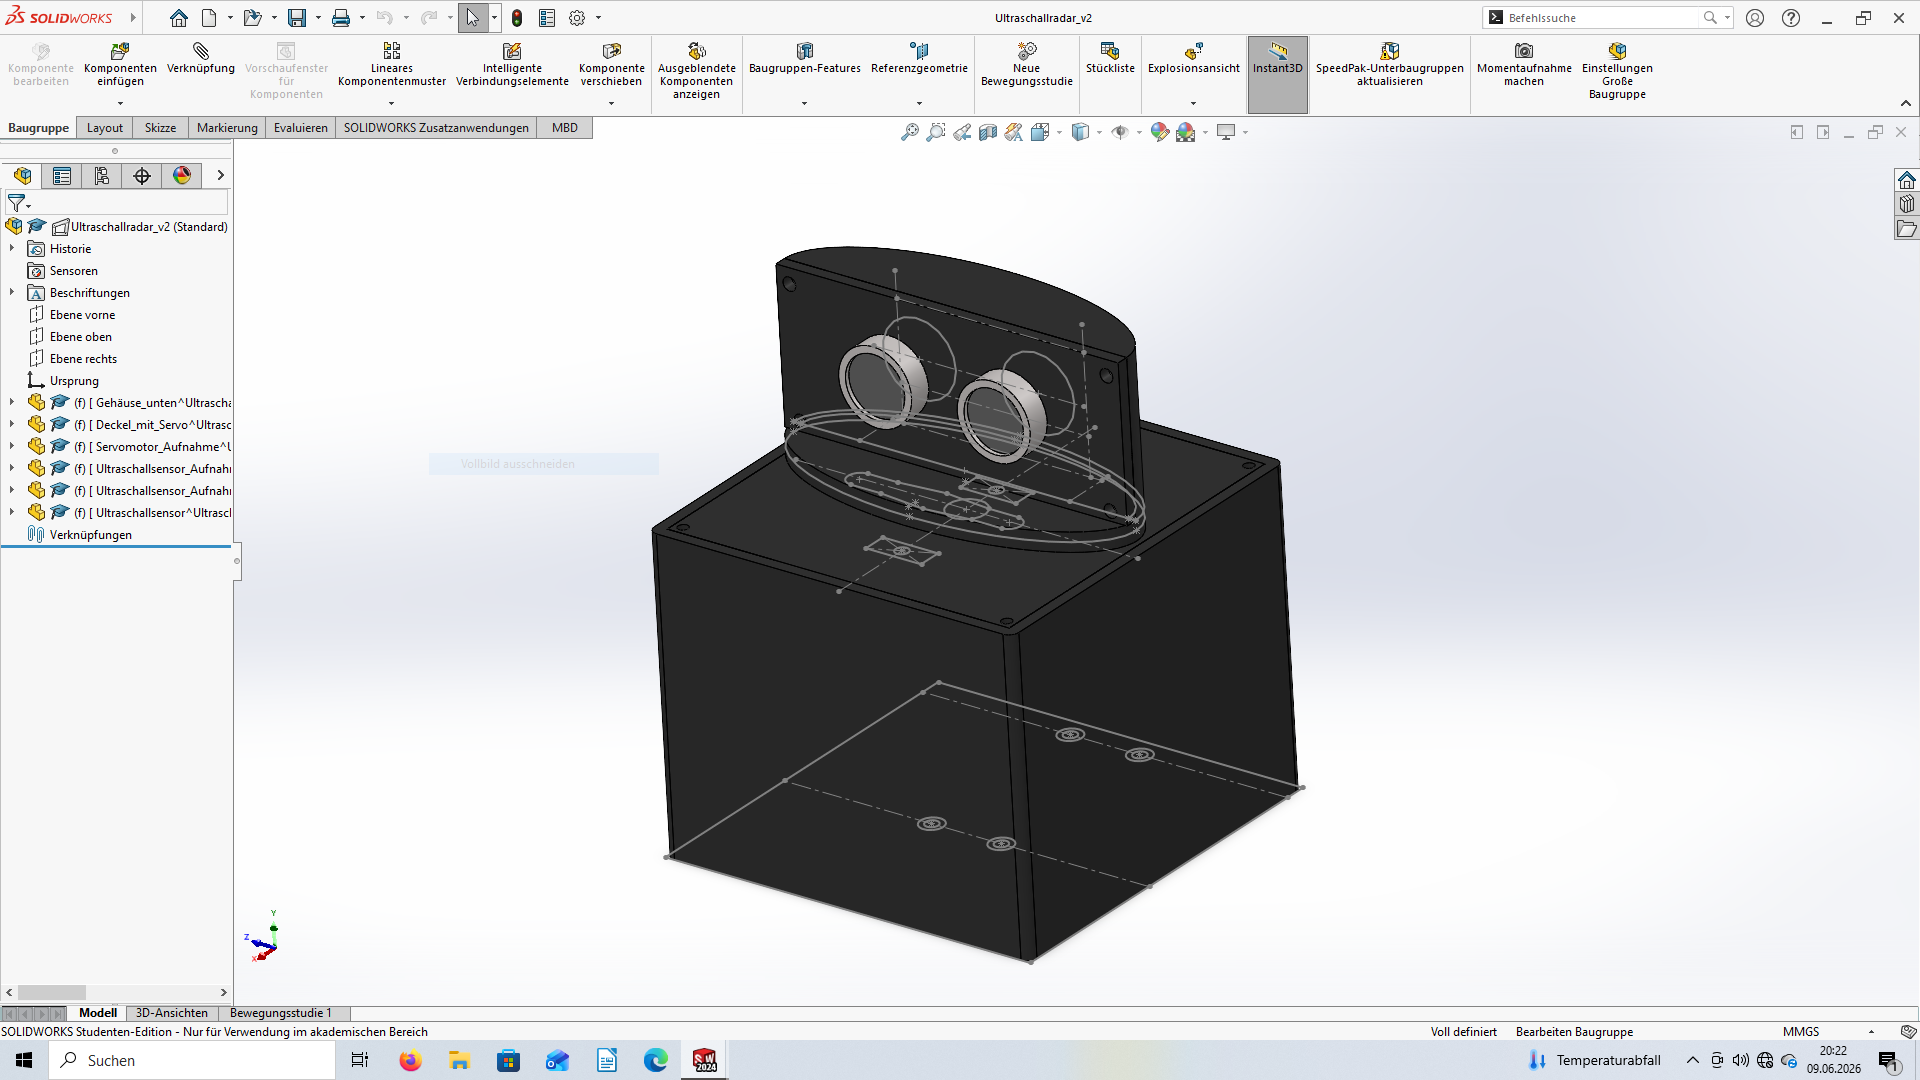
\includegraphics[width=\textwidth]{../Images/CAD/UltraschallradarCAD.PNG}
	\caption{Parametrische CAD-Baugruppe in SolidWorks: Invertierte Servomontage und zweiteiliges Gehäusedesign}
	\label{fig:CAD_SolidWorks_Baugruppe}
\end{figure}

Das mechatronische System wurde konstruktiv in vier separate Funktionselemente unterteilt:
\begin{enumerate}
	\item \textbf{Grundgehäuse:} Bildet die tragende Basisstruktur mit einer passgenauen Aussparung an der Frontseite für den USB-Anschluss des Arduino Nano sowie zwei präzisen Bohrungen für die optischen Status-LEDs (Rot und Grün).
	\item \textbf{Grundgehäusedeckel:} Deckelt das Grundgehäuse formschlüssig ab. Er verfügt an der Unterseite über eine integrierte, passgenaue Aufnahme des Servomotors sowie einen kreisbogenförmigen $180^\circ$-Drehspalt, durch welchen die Sensorleitungen kollisionsfrei geführt werden.
	\item \textbf{Sensoraufnahme:} Eine rotierende Aufsatzkomponente, welche die Geometrie der HC-SR04-Platine formschlüssig umschlie\ss t und mechanisch stützt.
	\item \textbf{Sensoraufnahmedeckel:} Schlie\ss t die rotierende Einheit ab und fixiert die Sensorplatine über exakte kreisrunde Ausschnitte für den Ultraschall-Sender und -Empfänger.
\end{enumerate}


\section{Mechatronischer Aufbau, Verbindungstechnik und Kabelmanagement}
\label{sec:Mechatronischer_Aufbau_Details}

Die mechanische und elektrische Systemintegration erfordert eine feste Verbindungstechnik, die dem zyklischen Wechselbetrieb der Drehbewegung standhält. Für alle kraft- und formschlüssigen Gehäuseverbindungen sowie für die Befestigung des Servomotors wurde ein einheitliches  Verbindungskonzept realisiert. In die konstruktiv berücksichtigten Verschrubungslöcher der 3D-Druckbauteile wurden mittels Hitze M2-Einschmelzmuttern aus Messing eingebracht. Die Fixierung der Deckelkomponenten und des Servomotors erfolgt über  M2-Inbus-Flachkopfschrauben, was eine zerstörungsfreie Demontage zu Wartungszwecken oder auch Reparaturarbeiten erlaubt.

\begin{figure}[htbp]
	\centering
	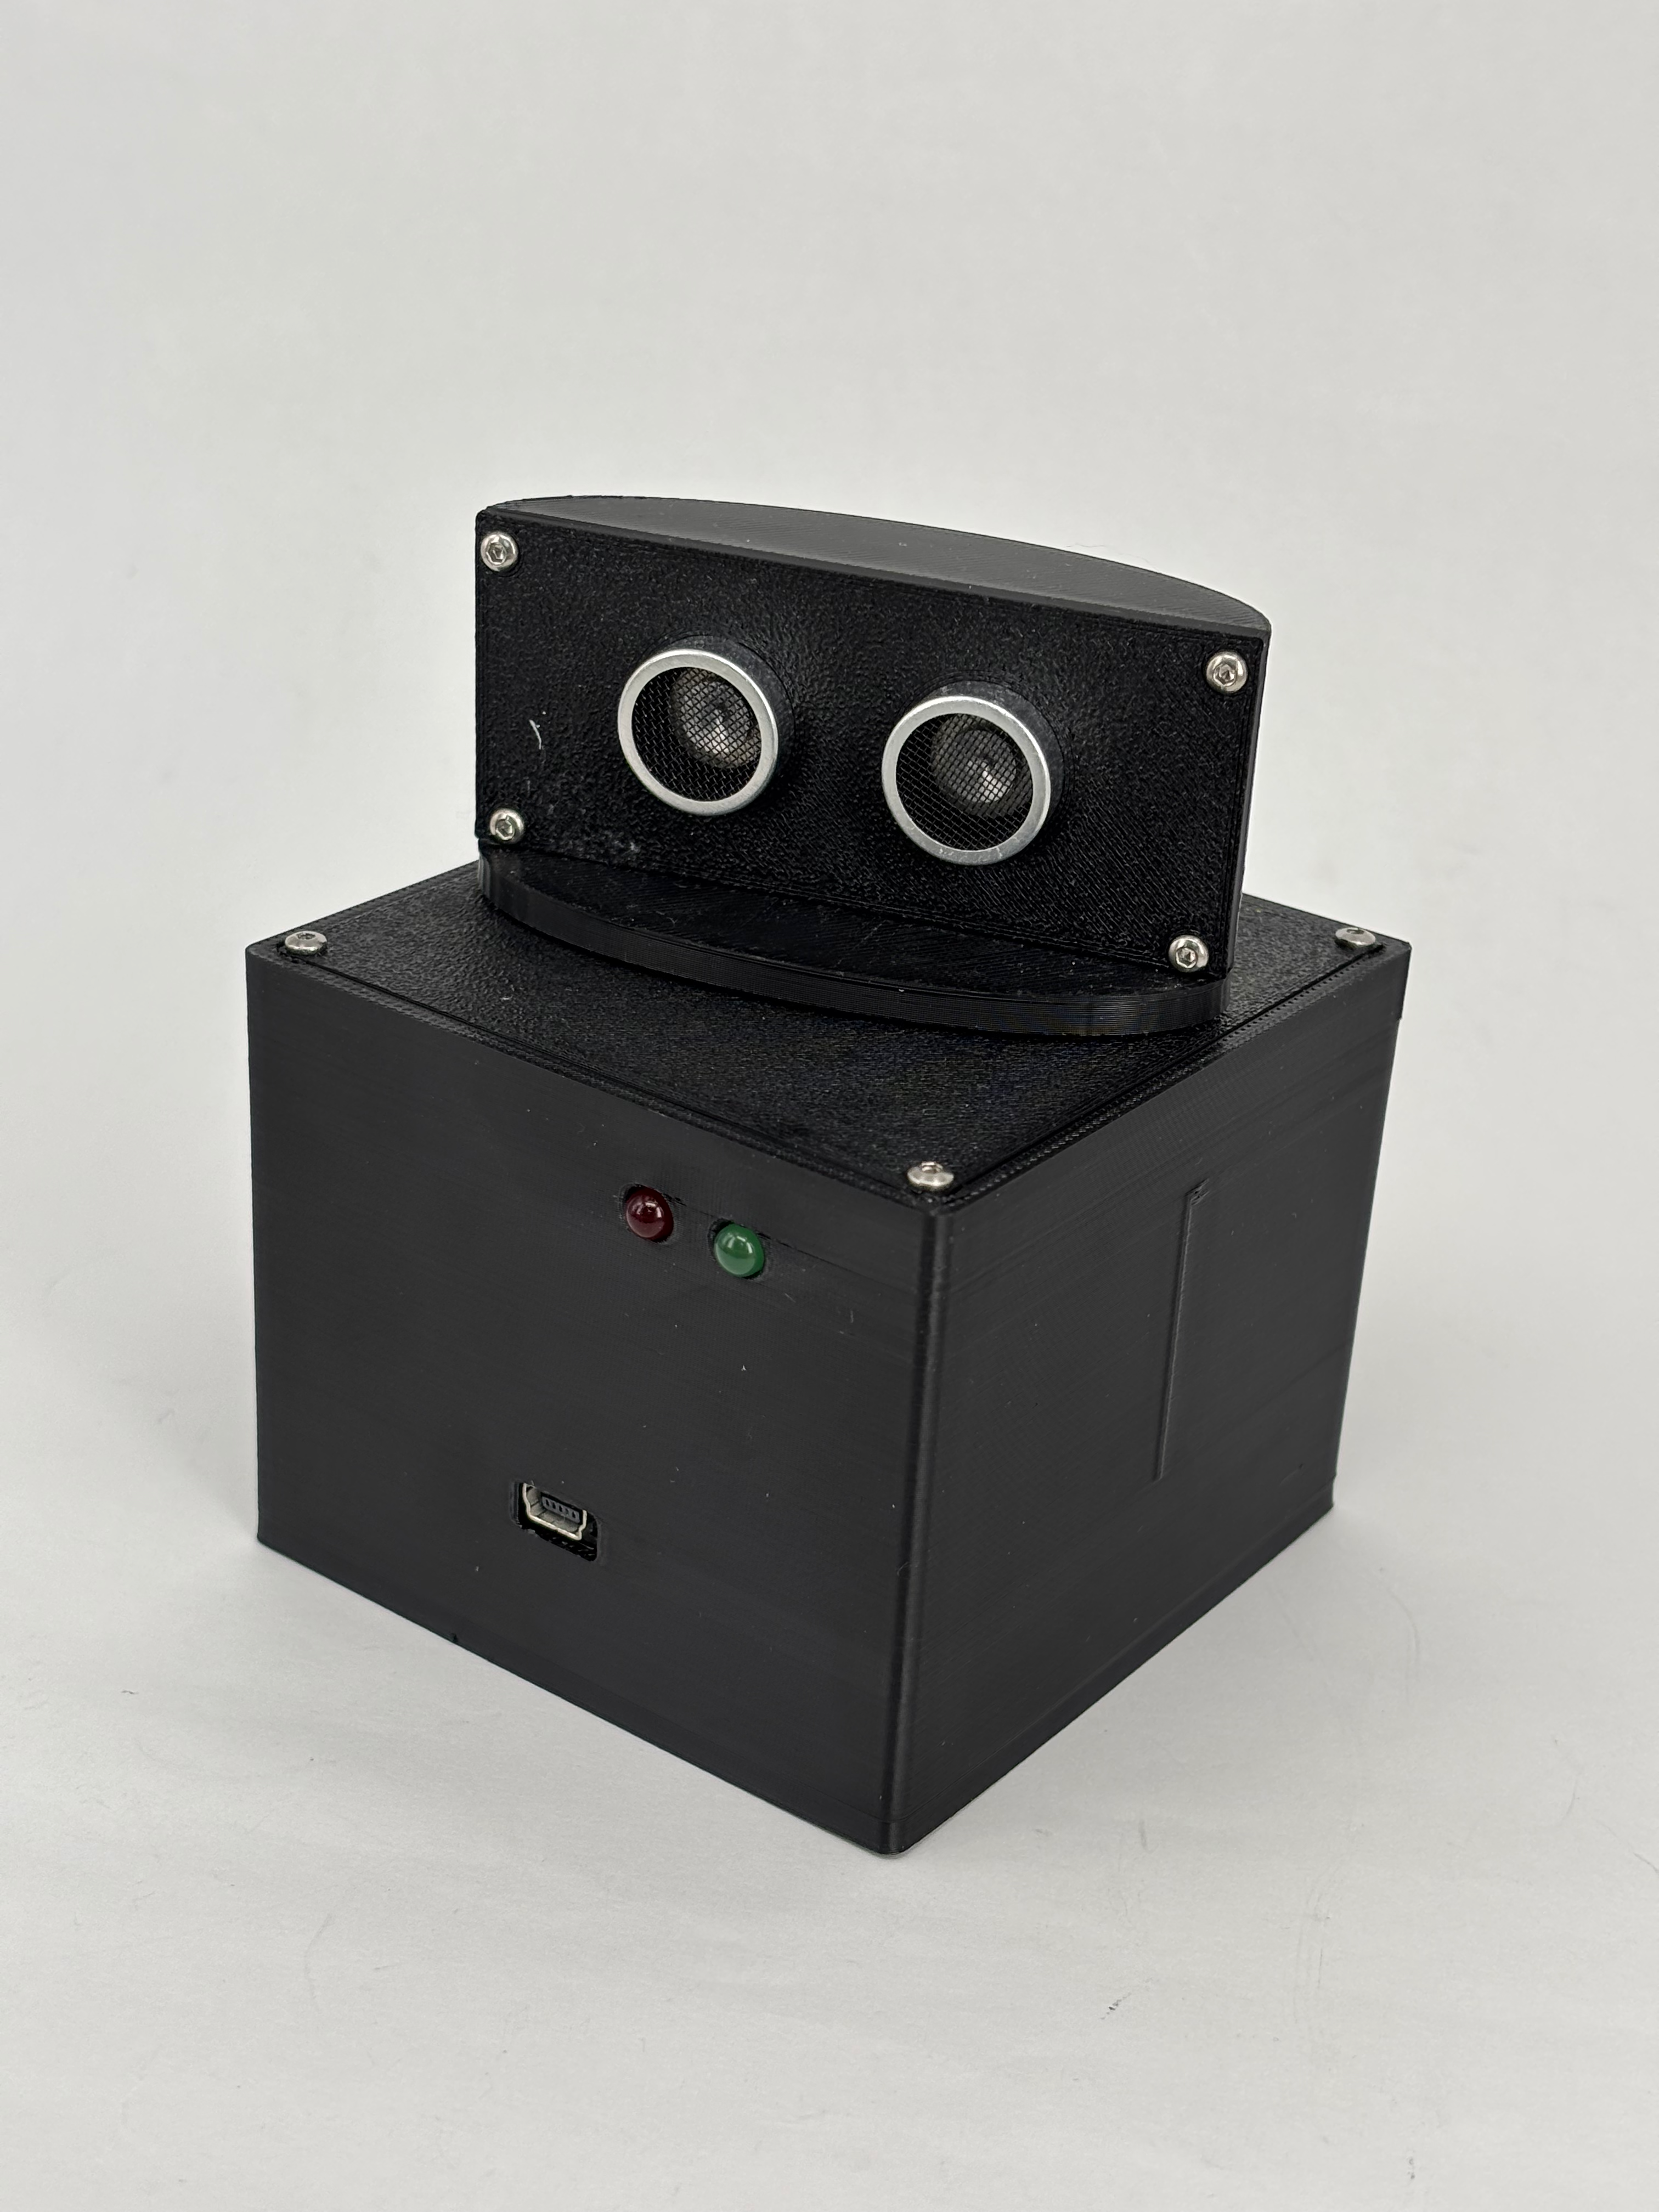
\includegraphics[width=\textwidth]{../Images/Fertigung/Ultraschallradarsystem.PNG}
	\caption{Ultraschallradarsystem mit integrierten Status-LEDs und verschraubten Gehäusekomponenten}
	\label{fig:Ultraschallradarsystem_Frontansicht}
\end{figure}

Der mechanische Kraftfluss wird realisiert, indem der TowerPro SG90 Servomotor von der Unterseite fest gegen den Hauptgehäusedeckel geschraubt wird. Nach dem bündigen Verschluss des Hauptgehäuses ist die verzahnte Abtriebswelle des Servos zum Aufstecken des Ultraschallsensors bereit. Auf diese profilierte Verzahnung wird die Sensoraufnahme axial aufgesteckt und damit formschlüssig gesichert. 

\begin{figure}[htbp]
	\centering	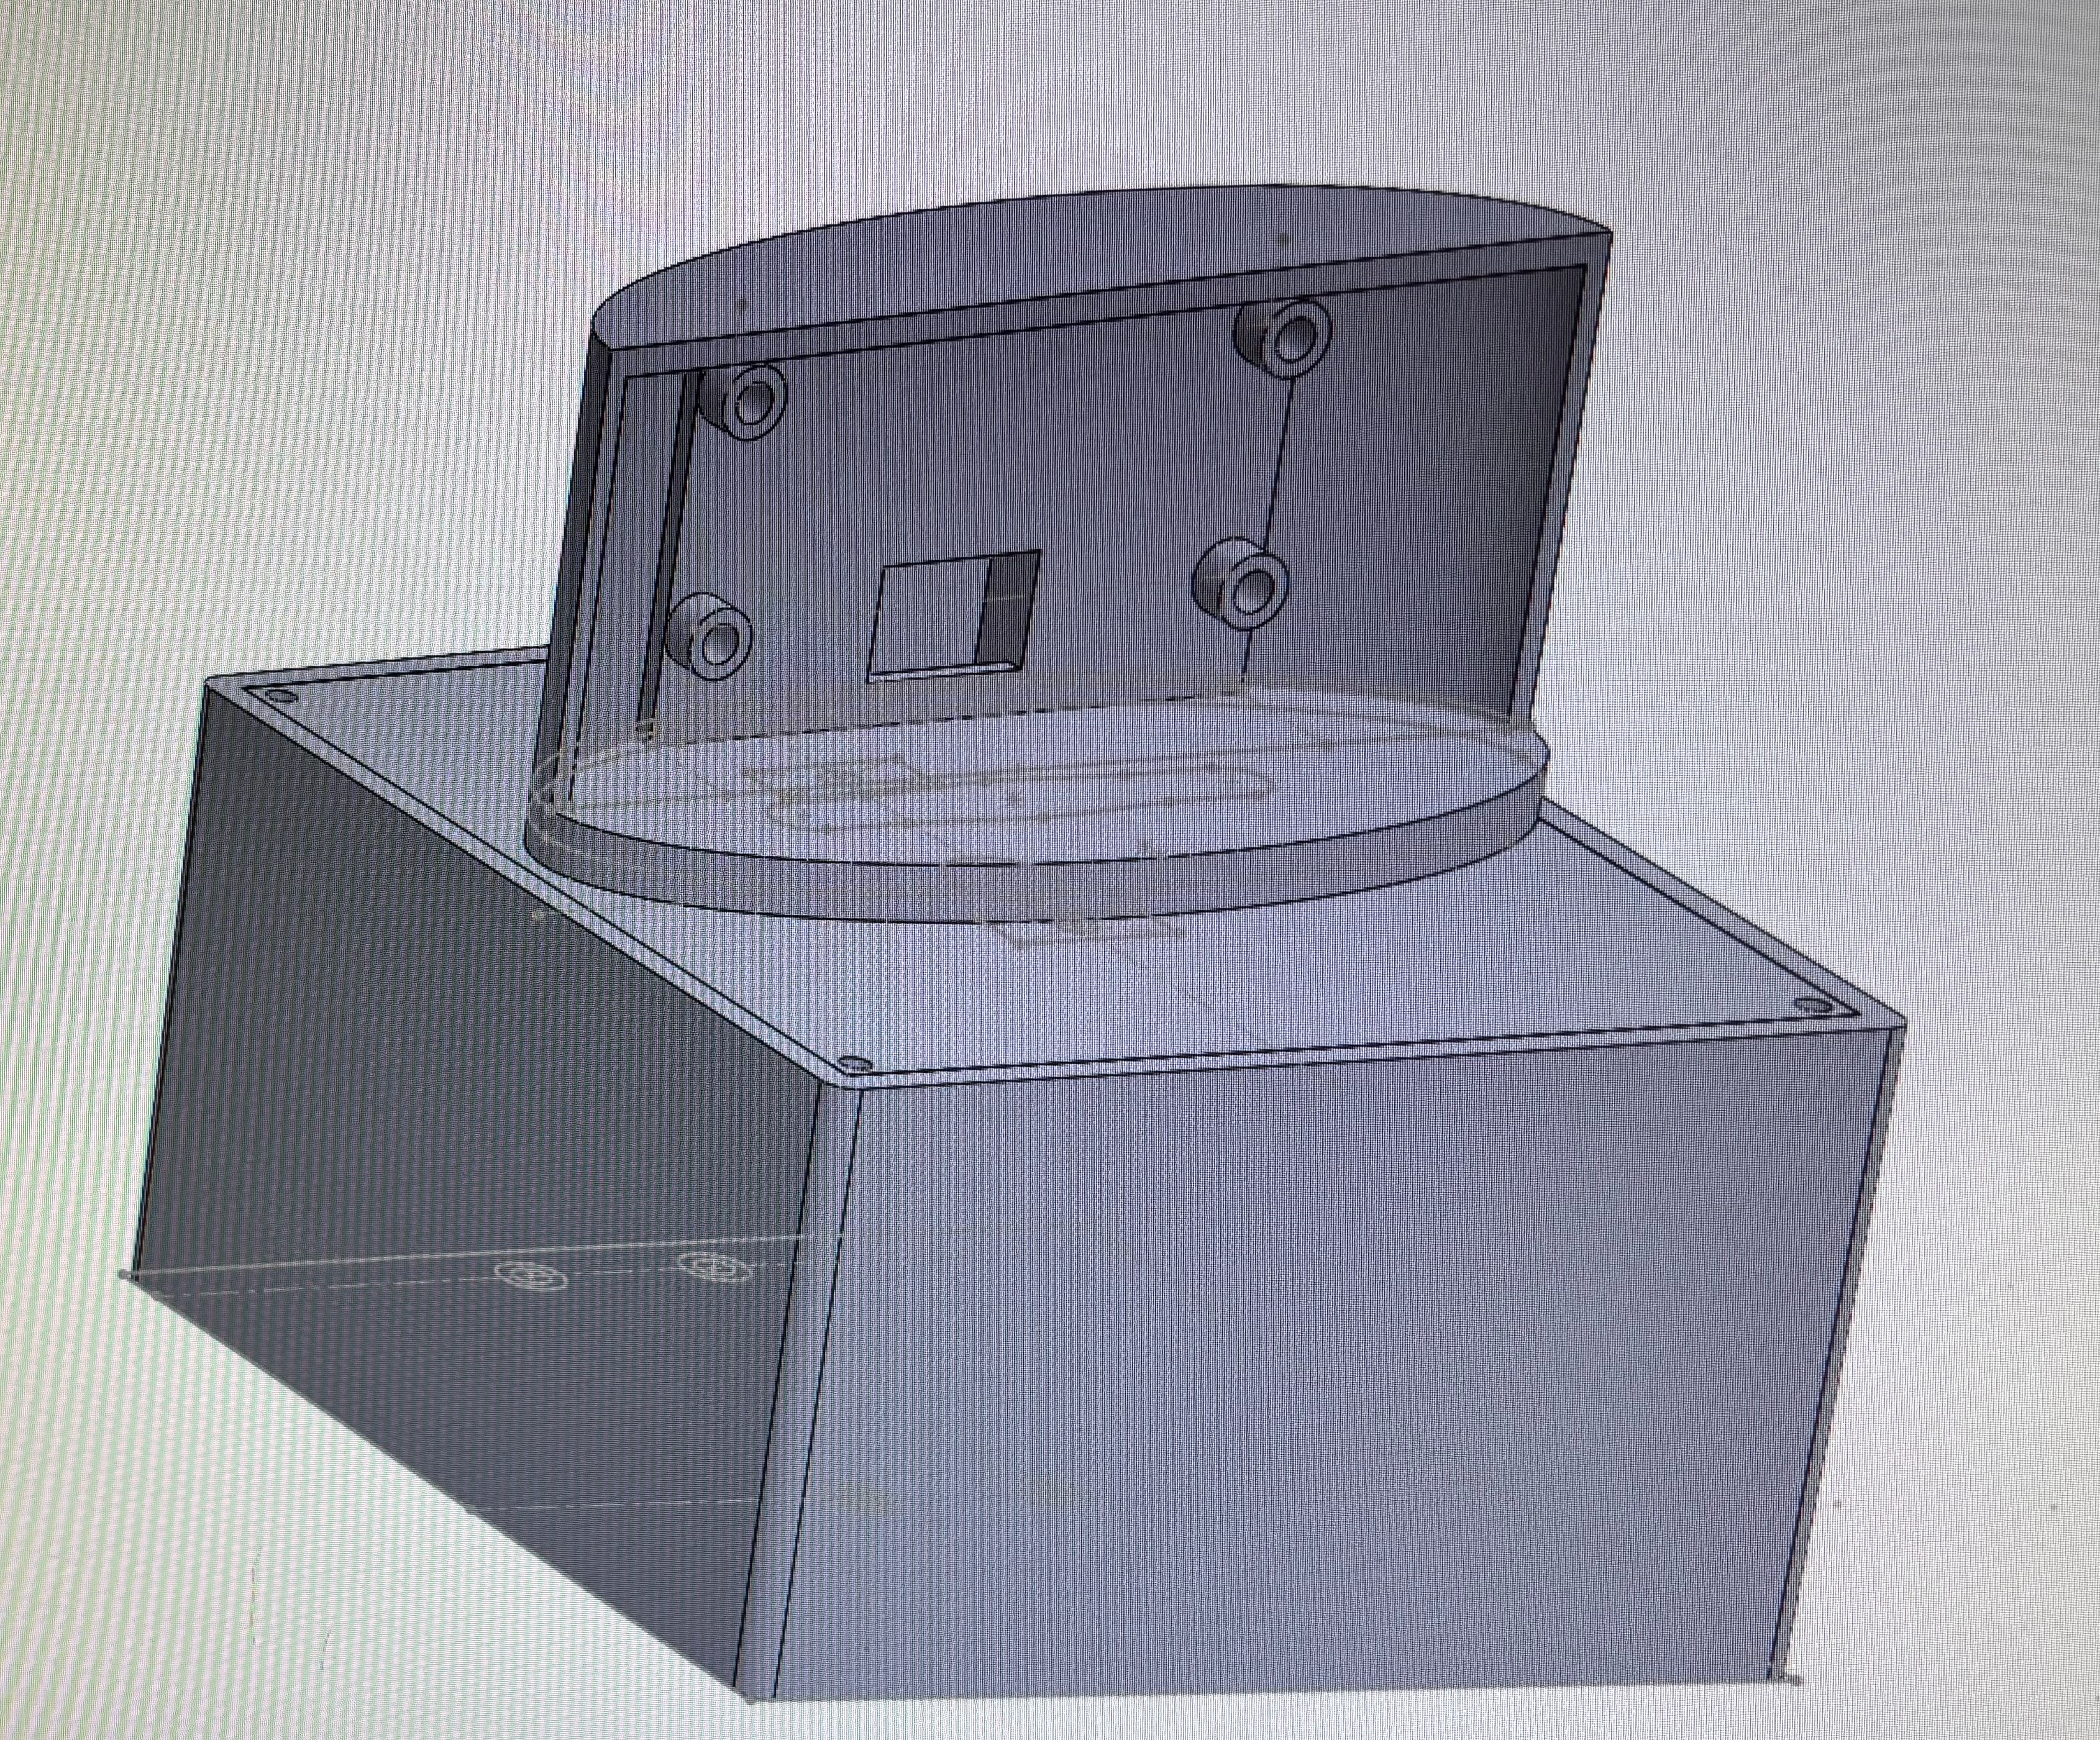
\includegraphics[width=0.55\textwidth]{../Images/Fertigung/InnenansichtSensoraufnahme.PNG}
	\caption{Innenansicht der Sensoraufnahme: Passgenaue HC-SR04-Aufnahme}
	\label{fig:Sensor_Verkabelung_Innen}
\end{figure}

Das elektrische System zeichnet sich durch ein volumenoptimiertes Kabelmanagement aus. Der Steuerungs-Mikrocontroller (Arduino Nano) ist im Grundgehäuse auf ein kompaktes 25-Pin-Mini-Breadboard gesteckt, welches das Zentrum der internen Signalverteilung bildet. Die Vorwiderstände für die Ansteuerung der roten und grünen Status-LEDs wurden direkt mit den Zuleitungen verlötet, isoliert und mit den digitalen GPIO-Pins des Mikrocontrollers verbunden. 

Um den Raumbedarf im Gehäuseinneren zu minimieren, wurden sämtliche internen Verbindungsleitungen auf das minimal notwendige Ma\ss  gekürzt. Eine kritische Ausnahme bildet hierbei der vieradrige Kabelstrang des HC-SR04-Ultraschallsensors: Dieser wurde exakt so dimensioniert, dass er im Gehäuseinneren eine flexible Schlaufe bildet. Diese Schlaufe stellt sicher, dass bei der oszillierenden $120^\circ$-Rotationsbewegung innerhalb des oberen $180^\circ$-Drehspalts ausreichend mechanisches Spiel vorhanden ist, um unzulässige Zugspannungen, Scheuereffekte oder Ermüdungsbrüche der Kabel dauerhaft zu verhindern.

Die vier Sensorleitungen werden im Gehäusedeckel direkt durch den kreisbogenförmigen $180^\circ$-Drehspalt in den Innenraum geführt. Dadurch erfährt der Kabelstrang bei der 120$^\circ$-Schwenkbewegung keine Biege- oder Zugbelastung. Kollisionen mit den Gehäuseinnenwänden oder ein Blockieren des Getriebes werden durch diese konstruktive Ma\ss nahme weitestgehend ausgeschlossen.

\section{Software-Architektur und Programmablaufpläne}
\label{sec:Software_Architektur_Protokoll}

Die Systemstabilität wird durch ein bidirektionales Kommunikationsprotokoll und zwei korrespondierende Zustandsmaschinen auf dem Mikrocontroller und der Processing-Applikation realisiert.

Anhand der softwareseitigen Implementierung wird die Systemstabilität durch zwei korrespondierende Zustandsmaschinen (Finite State Machines) auf dem Mikrocontroller sowie innerhalb der Processing-Applikation realisiert.

\begin{figure}[htbp]
	\centering
	\shorthandoff{"}
\begin{tikzpicture}[
	node distance=1.0cm,
	startstop/.style={rectangle, rounded corners=10pt, minimum width=3cm, minimum height=0.8cm, text width=3.5cm, align=center, draw=black, fill=gray!15, font=\sffamily\small},
	process/.style={rectangle, minimum width=3.5cm, minimum height=0.8cm, text width=3.8cm, align=center, draw=black, fill=blue!10, font=\sffamily\small},
	decision/.style={diamond, aspect=2, minimum width=3.5cm, minimum height=0.8cm, text width=2.8cm, align=center, draw=black, fill=yellow!15, font=\sffamily\small},
	errorbox/.style={rectangle, minimum width=3.5cm, minimum height=0.8cm, text width=3.8cm, align=center, draw=black, fill=red!15, font=\sffamily\small},
	arrow/.style={->, >=Stealth, thick}
	]
	
	% Knoten Definitionen
	\node (start) [startstop] {Start: Firmware Boot};
	\node (init) [process, below=of start] {Setup(): Initialisierung\\ \textbf{Rote LED = AN}};
	\node (dec1) [decision, below=of init] {Token \texttt{"P:START"} \\ empfangen?};
	\node (test) [process, below=of dec1] {\texttt{"S:TESTING"} senden\\ \textbf{Beide LEDs = AN}};
	\node (servo) [process, below=of test] {Servo auf 90$^\circ$ fahren\\ Testmessung auslösen};
	\node (dec2) [decision, below=of servo] {Messwert valide?\\ ($0 < d < 400\text{ cm}$)};
	\node (err) [errorbox, left=1.0cm of dec2] {Zustand \texttt{"S:ERR\_SENSOR"}\\ \textbf{Rote LED = AN}\\ \textit{Endlosschleife (Halt)}};
	\node (ok) [process, below=of dec2] {\texttt{"S:OK"} senden\\ \textbf{Grüne LED = AN}};
	\node (scan) [process, below=of ok] {loop(): Inkrementeller\\ Servo-Sweep (30$^\circ$--150$^\circ$)};
	\node (send) [process, below=of scan] {Telemetrie via UART:\\ \texttt{"D:Winkel,Distanz"}};
	
	% Pfeilverbindungen
	\draw [arrow] (start) -- (init);
	\draw [arrow] (init) -- (dec1);
	\draw [arrow] (dec1) -- node[anchor=west] {Ja} (test);
	\draw [arrow] (dec1.west) -- ++(-0.5,0) -- ++(0,1.5) -- node[anchor=south] {Nein} (init.west);
	\draw [arrow] (test) -- (servo);
	\draw [arrow] (servo) -- (dec2);
	\draw [arrow] (dec2) -- node[anchor=south] {Nein} (err);
	\draw [arrow] (dec2) -- node[anchor=west] {Ja} (ok);
	\draw [arrow] (ok) -- (scan);
	\draw [arrow] (scan) -- (send);
	\draw [arrow] (send.east) -- ++(0.5,0) -- ++(0,1.5) |- (scan.east);
	
\end{tikzpicture}
\shorthandon{"}
	\caption{Programmablaufplan (Flowchart) der eingebetteten Firmware auf dem Arduino Nano}
	\label{fig:Flowchart_Arduino}
\end{figure}

\begin{figure}[htbp]
	\centering
	\shorthandoff{"}
\begin{tikzpicture}[
	node distance=1.0cm,
	startstop/.style={rectangle, rounded corners=10pt, minimum width=3cm, minimum height=0.8cm, text width=3.5cm, align=center, draw=black, fill=gray!15, font=\sffamily\small},
	process/.style={rectangle, minimum width=3.5cm, minimum height=0.8cm, text width=3.8cm, align=center, draw=black, fill=green!10, font=\sffamily\small},
	decision/.style={diamond, aspect=2, minimum width=3.5cm, minimum height=0.8cm, text width=2.8cm, align=center, draw=black, fill=yellow!15, font=\sffamily\small},
	errorbox/.style={rectangle, minimum width=3.5cm, minimum height=0.8cm, text width=3.8cm, align=center, draw=black, fill=red!15, font=\sffamily\small},
	bootbox/.style={rectangle, minimum width=3.5cm, minimum height=0.8cm, text width=3.8cm, align=center, draw=black, fill=orange!15, font=\sffamily\small},
	arrow/.style={->, >=Stealth, thick}
	]
	
	% Knoten Definitionen
	\node (start) [startstop] {Start: Applikationsaufruf};
	\node (setup) [process, below=of start] {setup(): OS prüfen \&\\ COM-Ports auflisten};
	\node (dec1) [decision, below=of setup] {USB/COM Port\\ verfügbar?};
	\node (err) [errorbox, left=1.0cm of dec1] {\textbf{SYSTEMFEHLER}\\ Roter Warn-Screen\\ (Hintergrund-Polling)};
	\node (conn) [process, below=of dec1] {Port öffnen. Zyklisch\\ Token \texttt{"P:START"} senden};
	\node (dec2) [decision, below=of conn] {Eingehender\\ System-Status?};
	\node (boot) [bootbox, left=1.0cm of dec2] {Grauer Boot-Screen:\\ \textit{"System fährt hoch..."}};
	\node (live) [process, below=of dec2] {Status = \texttt{"OK"}\\ Radar HUD zeichnen\\ (Grid, Strahl, Text)};
	\node (watch) [decision, below=of live] {Watchdog aktiv:\\ Latenz $> 500$ ms?};
	\node (parse) [process, below=of watch] {\texttt{serialEvent()}: Parse Data\\ Hysteresefilter \&\\ Clusterbildung};
	
	% Pfeilverbindungen
	\draw [arrow] (start) -- (setup);
	\draw [arrow] (setup) -- (dec1);
	\draw [arrow] (dec1) -- node[anchor=west] {Ja} (conn);
	\draw [arrow] (dec1) -- node[anchor=south] {Nein} (err);
	\draw [arrow] (err) |- (setup);
	\draw [arrow] (conn) -- (dec2);
	\draw [arrow] (dec2) -- node[anchor=south] {\texttt{"TESTING"}} (boot);
	\draw [arrow] (boot.north) -- ++(0,1.5) |- (dec2.north);
	\draw [arrow] (dec2) -- node[anchor=west] {\texttt{"OK"}} (live);
	\draw [arrow] (live) -- (watch);
	\draw [arrow] (watch) -- node[anchor=west] {Nein} (parse);
	\draw [arrow] (watch.east) -- ++(0.5,0) |- (dec1.east) node[near end, anchor=south west, xshift=2pt] {Ja};
	\draw [arrow] (parse.west) -- ++(-0.5,0) -- ++(0,3.2) |- (live.west);
	
\end{tikzpicture}
\shorthandon{"}
	\caption{Programmablaufplan (Flowchart) der Visualisierungs- und Watchdog-Logik in Processing}
	\label{fig:Flowchart_Processing}
\end{figure}

Der Systemstart vollzieht sich über eine definierte Handshake-Sequenz, um ein unkontrolliertes Anlaufen der Hardware zu verhindern:
\begin{enumerate}
	\item \textbf{Initialisierung:} Nach dem Herstellen der Spannungsversorgung schaltet der Arduino die rote Status-LED ein und blockiert in einer dedizierten Warteschleife. Der Servo verbleibt starr.
	\item \textbf{Verbindungsaufbau:} Beim Öffnen der Processing-Applikation scannt diese plattformunabhängig die USB-Schnittstellen und sendet im 200-ms-Intervall den String \texttt{"P:START\textbackslash n"}.
	\item \textbf{Selbsttest (POST):} Nach Erhalt des Tokens bricht der Arduino aus der Warteschleife aus, signalisiert den Zustand \texttt{"S:TESTING"}, aktiviert beide Status-LEDs und fährt den Servo in die 90$^\circ$-Mittelstellung. Es folgt eine Testmessung mit dem Ultraschallsensor.
	\item \textbf{Normalbetrieb:} Ist die Testmessung gültig, schaltet der Arduino auf die grüne LED um, meldet \texttt{"S:OK"} und startet den kontinuierlichen Scan. Processing wechselt zeitgleich in die visuelle Radar-Oberfläche.
\end{enumerate}

\section{Algorithmische Signalaufbereitung und Clusterbildung}
\label{sec:Signalaufbereitung_Filter}

Um ein bestmögliches Abbild der Umgebung zu generieren und die physikalische Aufweitung des Ultraschall-Schallkegels zu kompensieren, findet in der Processing-Anwendung eine fortlaufende Filterung des Datenstroms statt.

\subsection{Laufzeit-Watchdog gegen Verbindungsverlust}
Zur Absicherung gegen Kabelbruch oder ein unvorhergesehenes Abstecken im laufenden Betrieb überwacht ein Software-Watchdog die Latenz der eintreffenden Datenpakete. Bei jedem Aufruf der seriellen Interrupt-Routine \texttt{serialEvent()} wird der Zeitstempel $t_{last}$ aktualisiert. Erreicht die Differenz zur aktuellen Systemzeit $t_{now}$ einen Schwellenwert von mehr als 500~ms:
\begin{equation}
	t_{now} - t_{last} > 500\text{ ms}
\end{equation}
wird die Verbindung sofort als unterbrochen klassifiziert. Die Anwendung schlie\ss t den toten Port sauber, schaltet augenblicklich auf den roten Systemfehler-Bildschirm um und startet die zyklische Hintergrundsuche nach der Hardware.

\subsection{Hysteresefilter und Clusterbildung}
Die Reduktion der virtuellen Objektverbreiterung, hervorgerufen durch den 15$^\circ$ breiten Schallkegel des HC-SR04, wird durch eine algorithmische Flankenerkennung realisiert. Der Filter analysiert die Abstände aufeinanderfolgender Winkelschritte ($i$ und $i-1$). Ein Objektübergang wird über eine empirisch ermittelte Distanz-Hysterese definiert:

\begin{equation}
	|d_i - d_{i-1}| > 3{,}5\text{ cm}
\end{equation}

Solange die Distanzänderung innerhalb dieser Hysteresegrenze verbleibt, werden die Messpunkte als zusammenhängendes mathematisches Cluster behandelt. Sobald der Schwellenwert von 3,5~cm überschritten wird, bricht der Algorithmus das aktuelle Cluster ab, berechnet das geometrische Zentrum sowie die gemittelte Objektdistanz und zeichnet das Hindernis als präzises, komprimiertes Kreissegment im UI. Signalfragmente mit einer Breite von weniger als 2$^\circ$ werden als statistisches Rauschen isoliert und vollständig verworfen.

\section{Implementierung und Quellcode-Analyse der Systemsoftware}
\label{sec:Software_Quellcode_Analyse}

Die mechatronische Funktionsfähigkeit des Radarsystems resultiert aus dem synchronisierten Zusammenspiel der eingebetteten Steuerungsebene auf dem Mikrocontroller und der grafischen Verarbeitungsebene der Desktop-Applikation. Zur Gewährleistung maximaler Transparenz und Modularität wurden beide Softwaremodule vollständig nach dem Doxygen-Dokumentationsstandard strukturiert. Die folgenden Abschnitte analysieren die strukturelle Architektur und algorithmische Funktionsweise der beiden Quellcodedateien.

\subsection{Detaillierte Analyse der Processing-Benutzeroberfläche}
\label{sec:Analyse_Processing_Code}

Die Benutzeroberfläche auf dem Host-Computer wird durch das in Java implementierte Skript realisiert. Die primäre Aufgabe dieser Anwendung besteht darin, als grafisches Terminal zu fungieren, den Systemzustand visuell zu überwachen und die eintreffenden Sensor-Rohwerte in ein euklidisches Koordinatensystem zu überführen.

Der vollständige, plattformunabhängige Quellcode der Benutzeroberfläche ist in Listing~\ref{lst:Processing_Code} dokumentiert.

\begin{center}
	\captionof{code}{UltraschallradarProcessing} 
	\label{code:UltraschallradarProcessing} \ArduinoExternal{}{../../Code/Processing/BenutzeroberflaecheV2.pde} 
\end{center}


\bigskip
\noindent
\textbf{Strukturelle und algorithmische Funktionsbeschreibung des Frontend-Codes:}

\begin{itemize}
	\item \textbf{Globale Datenstrukturen und Puffer:} Auf globaler Ebene wird die serielle Kommunikationspipeline über die Instanz \PYTHON{myPort} verwaltet[cite: 5]. Der systemweite Ablauf wird durch eine Zustandsmaschine kontrolliert, welche die diskreten Zustände \texttt{BOOT}, \texttt{TESTING}, \texttt{OK}, \texttt{ERR\_PORT} und \texttt{ERR\_SENSOR} einnehmen kann[cite: 5]. Für die Erzeugung des charakteristischen Nachleuchteffekts der Radar-Anzeige (Phosphor-Glow) sorgt das Fließkomma-Array \PYTHON{radarWerte}, welches 181 Speicherzellen umfasst und über den gemessenen Azimutwinkel als Direktzugriffsindex adressiert wird[cite: 12, 13].
	\item \textbf{System-Initialisierung (\PYTHON{setup}):} Beim Programmstart erzwingt die Routine \PYTHON{setup()} die Ausführung im nativen Fullscreen-Modus des Host-Rechners[cite: 17, 18]. Zur visuellen Kantenglättung der Vektorgrafiken werden hardwareseitige Anti-Aliasing-Pipelines aktiviert[cite: 19]. Die Geometrie des Radar-Anzeigeradius wird hierbei dynamisch und adaptiv auf exakt 65\,\% der vertikalen Bildschirmhöhe skaliert, wodurch sich das UI flexibel an unterschiedliche Monitorauflösungen anpasst[cite: 10, 19].
	\item \textbf{Kommunikationsaufbau (\PYTHON{connectSerial}):} Die Methode kapselt den Eröffnungshook der seriellen Hardware-Schnittstelle[cite: 21]. Um I/O-Abstürze des Betriebssystems bei unvollständigen Datenpaketen oder während des Hot-Plugging-Betriebs zu verhindern, ist die Instanziierung in einen Try-Catch-Block eingebettet[cite: 23, 24]. Der serielle Empfangspuffer wird explizit angewiesen, den asynchronen Interrupt erst beim Eintreffen eines vollständigen Zeilenumbruchs (\texttt{'\textbackslash n'}) auszulösen[cite: 24, 25].
	\item \textbf{Die grafische Render-Schleife (\PYTHON{draw}):} Die Funktion \PYTHON{draw()} arbeitet als sequenzielle Weiche zur Darstellung der unterschiedlichen GUI-Ebenen[cite: 28]. Liegt ein Verbindungsfehler vor, wird das Rendern blockiert und ein tiefroter Systemfehler-Bildschirm ausgegeben[cite: 29, 30, 31]. Innerhalb dieses Fehlerzustands läuft eine automatisierte Hintergrundschleife, die alle 2000 Millisekunden einen erneuten Verbindungsversuch zur Hardware initiiert[cite: 32]. Im Zustand \texttt{BOOT} schaltet das UI auf ein anthrazitgraues Layout um und sendet im 200-ms-Takt das Token \texttt{"P:START\textbackslash n"}, um den Arduino aus seinem Boot-Block zu befreien[cite: 36, 37, 39]. 
	\item \textbf{Watchdog-Überwachung und Radar-Matrix:} Im aktiven Live-Modus (\texttt{OK}) überwacht die Schleife fortlaufend den Software-Watchdog[cite: 42]. Sollte die Differenz zur letzten erfolgreichen Datenübertragung (\PYTHON{lastDataReceivedTime}) das kritische Zeitfenster von 500 Millisekunden überschreiten, bricht das System die Verbindung ab und schützt sich vor unkontrollierten Zuständen[cite: 42, 43]. Die Darstellung des taktischen HUDs erfolgt über eine translationale Verschiebung des Koordinatensystems in das untere mathematische Zentrum des Bildschirms[cite: 44, 45].
	\item \textbf{Algorithmische Signalfilterung und Clusterbildung:} Zur Eliminierung von transientem Rauschen und zur Kompensation der physikalischen Schallkegelaufweitung durchläuft der Datenstrom eine Flankenerkennung[cite: 3, 54, 75]. Das System iteriert durch das Sensor-Array[cite: 56]. Wenn die Distanzänderung zwischen benachbarten Winkelschritten den Hysterese-Schwellenwert von 3,5~cm überschreitet, wird die aktuelle Datenreihe separiert und als zusammenhängendes Objekt-Cluster interpretiert[cite: 3, 59]. Die Funktion \PYTHON{drawCompensatedObject()} berechnet daraufhin den realen Schwerpunkt und zeichnet schmale Hindernisse als fokussierte Vektor-Ellipse, während breite Oberflächen als kontinuierliches, kreisbogenförmiges Kreissegment dargestellt werden[cite: 69, 70, 71, 75].
	\item \textbf{Serieller Daten-Parser (\PYTHON{serialEvent}):} Der serielle Interrupt verarbeitet eingehende Zeichenketten entkoppelt vom Grafik-Thread[cite: 81, 84]. Er extrahiert die System-Header: Statusmeldungen mit dem Präfix \texttt{"S:"} aktualisieren die globale Zustandsmaschine, während Telemetriedaten mit dem Präfix \texttt{"D:"} über eine String-Splittung in Winkel und Distanz zerlegt und im Daten-Array abgespeichert werden[cite: 82, 87, 89, 91].
\end{itemize}


\subsection{Detaillierte Analyse der Arduino-Firmware}
\label{sec:Analyse_Arduino_Code}

Die Firmware des Mikrocontrollers stellt das eingebettete Echtzeit-Kontrollzentrum des Radarsystems dar. Ihre primäre Aufgabe ist die präzise Ansteuerung des Pulsweitenmodulations-Signals (PWM) für den Servomotor, die zeitkritische Erzeugung und Erfassung der Ultraschallwellen sowie die Strukturierung des seriellen Datenstroms.

Der vollständige Quellcode der Firmware ist in Listing~\ref{lst:Arduino_Code} dokumentiert.

\begin{center}
	\captionof{code}{UltraschallradarArduino} 
	\label{code:UltraschallradarArduino} \ArduinoExternal{}{../../Code/Arduino/Ultraschallradar/UltraschallradarArduinoIDEMitDoxygen/UltraschallradarDoxygen.ino} 
\end{center}

\bigskip
\noindent
\textbf{Strukturelle und algorithmische Funktionsbeschreibung des Firmware-Codes:}

\begin{itemize}
	\item \textbf{Hardware-Mapping und Pin-Konfiguration:} Das Skript deklariert die physikalische Pinbelegung des Arduino Nano[cite: 95]. Über die digitalen GPIO-Pins 2 und 3 werden die zweifarbigen Status-LEDs (Grün für Betriebsbereitschaft, Rot für Fehler/Wartezustand) angesteuert[cite: 100, 101]. Die Pins 4 und 5 steuern die Ultraschall-Peripherie (Trigger-Ausgang und Echo-Eingang) [cite: 102, 103], während Pin 9 als dedizierter Timer-Ausgang für die präzise Winkelpositionierung des SG90-Servomotors über die hardwarenahe \texttt{Servo}-Bibliothek konfiguriert ist[cite: 104, 105].
	\item \textbf{Die Boot- und Handshake-Phase:} Nach dem Einschalten der Betriebsspannung setzt die \PYTHON{setup()}-Routine das System in einen sicheren Ausgangszustand[cite: 106]. Die serielle UART-Schnittstelle wird auf eine feste Übertragungsgeschwindigkeit von 9600 Baud initialisiert[cite: 107, 111]. Sofort wird die rote Status-LED aktiviert und die grüne LED abgeschaltet[cite: 108, 113]. Das System blockiert nun in einer permanenten \PYTHON{while(true)}-Schleife und verbleibt im passiven Zustand, bis das exakte Handshake-Signal \texttt{"P:START"} vom PC-Frontend empfangen wird[cite: 97, 114, 115]. Diese Verriegelung verhindert unkontrollierte mechanische Bewegungen beim Systemstart[cite: 97].
	\item \textbf{Power-On Self-Test (POST) und Soft-Startup:} Sobald die Verbindung steht, signalisiert der Arduino den Zustand \texttt{"S:TESTING"} an den PC und schaltet beide LEDs gleichzeitig ein[cite: 96, 116, 117]. Um das mechanische Servogetriebe vor plötzlichen Stromspitzen und abrupten Beschleunigungen zu schützen, liest die Firmware den aktuellen Ist-Winkel aus und führt einen sanft beschleunigten \PYTHON{for}-Schleifen-Sweep durch, um den Sensor materialschonend in die $90^\circ$-Mittelstellung zu bewegen[cite: 97, 117, 119, 120]. Anschließend wird eine einzelne Testmessung zur Hardware-Diagnose ausgelöst[cite: 97, 109, 121]. Liefert der Sensor ein plausibles Ergebnis innerhalb der physikalischen Grenzen von 0 bis 400~cm, schaltet das System die rote LED aus, aktiviert die grüne LED und gibt die Hauptschleife frei[cite: 110, 123, 124]. Ein Fehlersignal hingegen arretiert das System dauerhaft in einer defensiven Endlosschleife zum Schutz der Hardware[cite: 111, 125].
	\item \textbf{Die symmetrische Sweep-Kinematik (\PYTHON{loop}):} Die kontinuierliche Hauptschleife \PYTHON{loop()} steuert die raumbezogene Erfassung[cite: 125, 129]. Um mechanische Umkehrschwingungen und abrupte Richtungswechsel des Servos zu minimieren, ist der Schwenkbereich von $120^\circ$ (zwischen $30^\circ$ und $150^\circ$) in drei harmonisch aufeinander abgestimmte Phasen unterteilt: eine Zentrierungsphase ($90^\circ$ bis $30^\circ$), ein vollständiger Vorwärts-Sweep ($30^\circ$ bis $150^\circ$) und eine Rückholphase ($150^\circ$ zurück zur Mitte auf $90^\circ$)[cite: 126, 127, 128, 129, 130, 131].
	\item \textbf{Datenerfassung und Telemetrie-Export (\PYTHON{scanPosition}):} Das Herzstück der Messwerterfassung bildet das Unterprogramm \PYTHON{scanPosition()}[cite: 132, 137]. Nach jedem inkrementellen Winkelschritt blockiert die Firmware die Ausführung für exakt 35 Millisekunden[cite: 134, 138]. Dieses mechanische Beruhigungszeitfenster ist zwingend erforderlich, damit die durch den Stopp-Befehl des Servos induzierten Mikro-Vibrationen des Gehäuses abklingen können, bevor die Messung startet; dies verhindert ein visuelles Jitter-Zittern im GUI[cite: 134, 138]. Der Ultraschall-Messzyklus wird durch einen präzisen 10-Mikrosekunden-High-Impuls am Trigger-Pin initiiert[cite: 138, 139]. Die anschließende Laufzeitmessung des Echos wird über die mathematische Konstante der Schallgeschwindigkeit umgerechnet[cite: 135, 140]. Schließlich formatiert der Mikrocontroller den Datensatz in den synchronisierten Daten-String \texttt{"D:[Winkel],[Distanz]"} und sendet ihn über den UART-Bus an den PC[cite: 98, 136].
\end{itemize}